\chapter{Prototype \#2}

This chapter describes the chronology of this project's second prototype...

\section{Conception}

This prototype's purpose was to explore possible input mechanisms for audience members. Through user testing, I hoped to identify which were intuitive, which were most natural and meaningful to perform as a group, and which afforded accurate collaborative control. From the start, it was clear that body movement would be more a fitting input than something like button pressing. Users find movement-based interactions more satisfying (Ulyate \& Biancardi, 2001); furthermore, there are apparent subconscious ties that link music and movement (Jourdain, 1997; Levitin, 2006), making this a natural form of input for a live music environment. In designing their audience-interaction system, Barkhuus and Jorgensen (2008) found that movements based on already-present behaviour were especially effective input methods. Inspired by this recommendation, I created a list of common crowd behaviours to be incorporated in the system -- giving a thumbs up or thumbs down, swaying one's arms back and forth, clapping, doing `the wave,' holding a lighter in the air, and dancing. Researchers emphasize the importance of meaningful feedback in crowd-controlled systems (Ulyate \& Biancardi, 2001; Barkhuus \& Jorgensen, 2008), and this was also a recurring concern in the response to Prototype \#1. Thus, this prototype also allowed for exploration of different feedback methods. After receiving the opportunity to participate in an exhibition at OCAD University, I decided to design this prototype as an interactive installation. By inviting the exhibition attendees to test the various methods of input, I could observe the behaviours of a wide variety of users.

% Background:
% Auslander, 1999: Communities are formed based on how the audience interacts, with no dependence on the spectacle at hand
% Turino, 2008:
% * Artists can shift between participatory and presentational performance
% * Different roles of different difficult allow for everyone to feel welcome and achieve flow. "Core" and "elaboration" roles cater to advanced and non-advanced performers respectively.
% * Open form: Basic motives repeated over and over. Easy for newcomers to join in. "Security in constancy." Can facilitate flow.
% * Hall: Repetition can increase intensity. Synchronicity comforts people.
% * Wide tuning, loud volumes, and overlapping textures provide a ``cloaking function'' that makes people more comfortable participating
% * Virtuosic solos are not common
% * Some participatory performances are sequential -- everyone gets a turn (e.g. Karaoke)
% Kelly, 2007: Displaying clips and themes from her music videos at a Madonna concert creates feelings of a "shared past" in the audience. (How might we create instead a "shared present"?)
% Small, 1998: Performers dressing in uniform are separating themselves and their responsibilities
% Davidson, 1997:
% * Performance etiquette is usually formed by crowd mentality, following the majority
% * Performers pick up information from the audience's broad and specific behaviours
% * Visuals help audiences read the performer's intentions
% Sexton, 2007: Simple synchronous interactions in sound art projects left users with little to explore, resulting in a "flat" experience
% Jourdain, 1997: We move to music in order to "represent" it. This also amplifies, resonates the musical experience.
% Levitin, 2006:
% * "In every society of which we're aware, music and dance are inseparable." Ancient music was based on rhythm and movement. Combining rhythm and melody bridges our cerebellum and cerebral cortex.
% * Ties between music and movement have only been minimized in the last 100 years
% Kelly, 2007: Technology incorporated into a show can either be addressed as part of the show or hidden and made illusory
% Maynes-Aminzade, 2002:
% * Computer vision: Movement-based control were intuitive, but camera required frequent calibration
% * Beach ball: Using a single beach ball as an input was also intuitive, but it only involved a few people at a time
% * Laser pointers: Gave everyone an individual cursor, but got chaotic once more and more people joined
% * Recommendations: Focus on compelling activity over impressive technology. Not everyone must be sensed as long as they feel involved. The control mechanism should be obvious or the users will give up. Make the activity emotionally engaging. Emphasize cooperation.
% Ulyate, 2001:
% * Design guidelines:
% * * Encourage and reward movement
% * * Feedback should be immediate, obvious, and meaningful in the context of the space
% * * No instruction or thinking should be required
% * * Responsiveness is more important than aesthetics
% * *  Modularity is key
% * Lessons learned:
% * * Full-body movement is most satisfying
% * * Form of the object determines how users interact
% * * A practical system is distributed and scalable
% * * Find balance between freedom and constraint
% * * Users will always find a way to create unwanted outputs
% * * Simple, instant gratification is important for feedback
% Barkhuus, 2008:
% * Inputs based on already-present behaviour lead to intuitive systems
% * Don't focus on employing cutting edge technology
% * Events should not rely on the success of the technology
% * Immediate visual or aural feedback is key
% Tseng, 2012: Being excluded from the interaction did not lessen enjoyment of the show
% Reeves, 2010:
% * "Intra-crowd interaction" is a common phenomena to exploit
% * Many actions "snowball" and overtake crowds; highly visible/audible actions promote this
% * People on the fringes of the crowd interact, but there is latency
% * Every crowd is different; designs should reflect the environment
% Gates, 2006: Technologies should reflect the performer's art and not be a burden on them


\section{Prototyping}

The first prototype provided a suitable framework for this experiment: I continued using multiple Wii controllers as input devices, and OSCulator was used to route the data to Max where it processed and represented visually. From here, I needed to be able to recognize when a user was performing one of the selected crowd behaviours. By pulling data from the controller's motion sensors, I was able to identify when the user was giving a thumbs up or down, swaying their arms left or right, clapping, or doing the wave. I incorporated simple visual feedback -- LED objects that light up when the user holds their thumb up or down or claps, sliders that follow arm movement when the user is swaying or doing the wave. Calibrating these required trial and error tests using different thresholds -- determining what amount of acceleration qualified as a clap, for instance. Figure \ref{prototyping2.1} shows the first iteration of this prototype.

\begin{figure}[t]
	\centering

	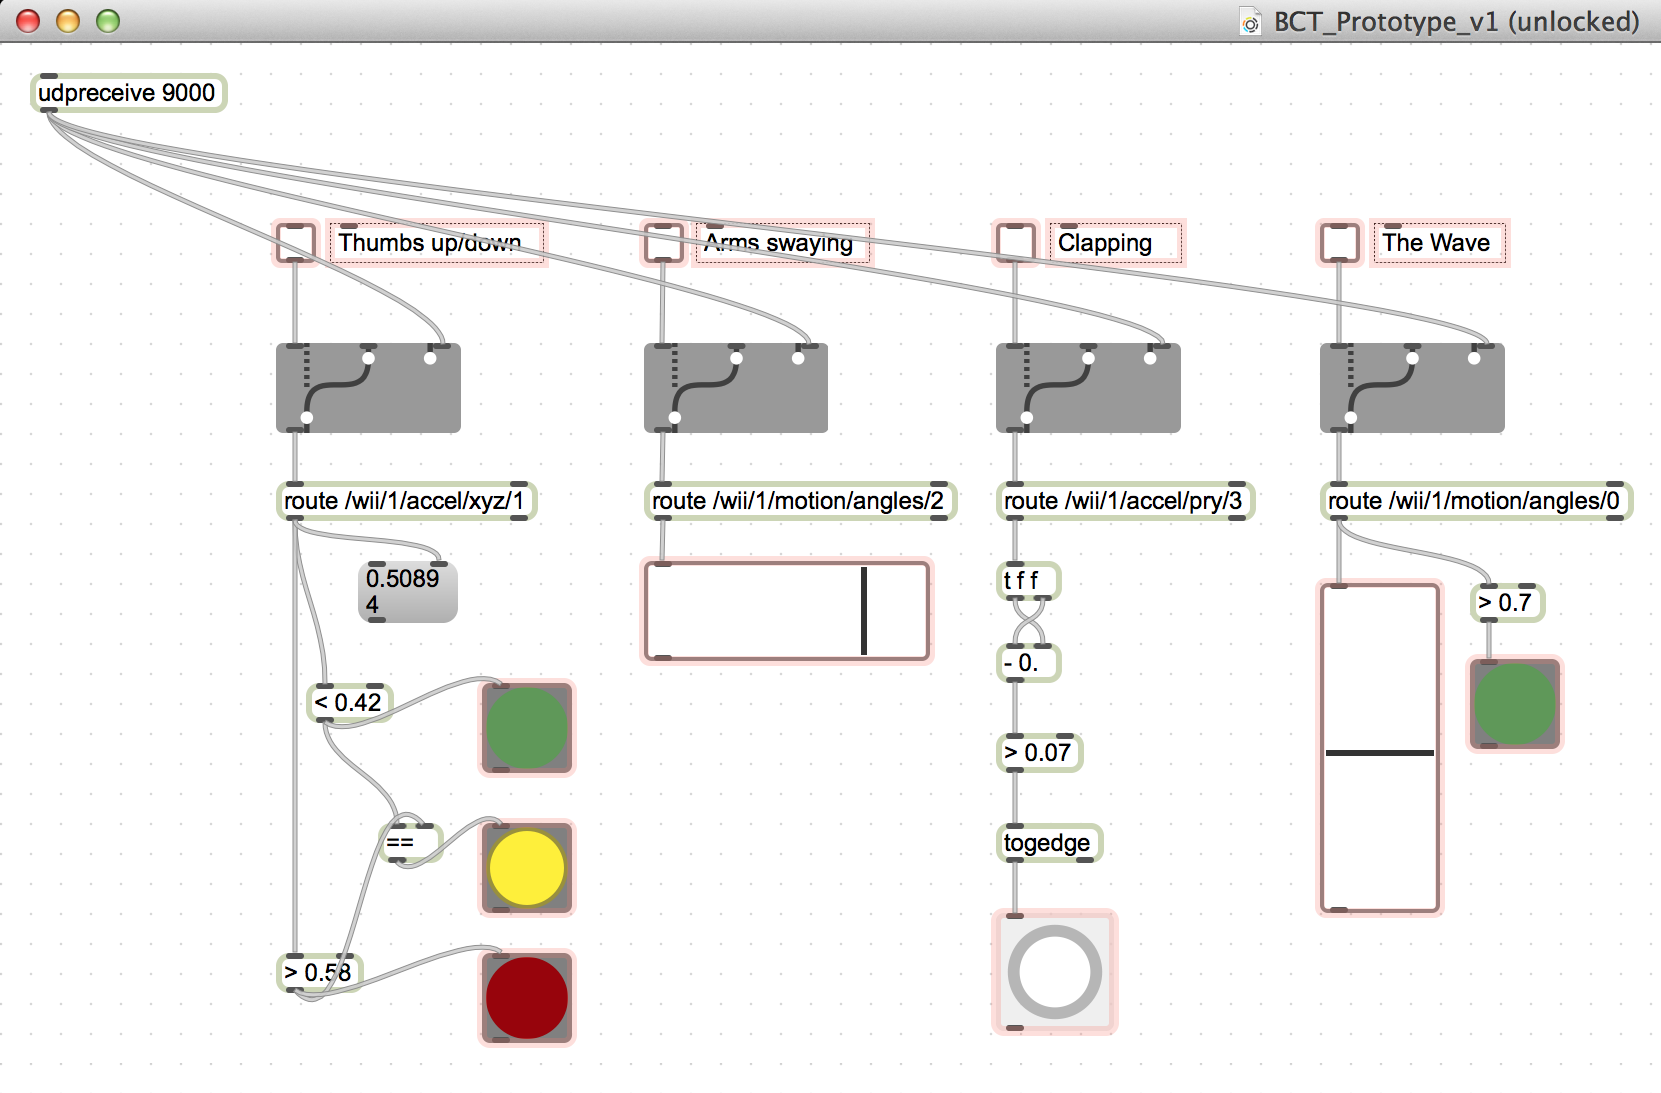
\includegraphics[height=0.4\textwidth]{wiimote_audience.png}
	\caption{Monitoring thumbs up/down, arm swaying, clapping, and the wave}

	\label{prototyping2.1}
\end{figure}

Next, I modularized the previous patcher and multiplied it sevenfold. The actions of seven users could now be monitored simultaneously. I developed new visualizations to reflect these multiple inputs, shown in Figure X. Thumbs up/down mode simply displays how many users are holding their thumbs up and down. The wave mode shows the vertical position of each user's arms. I created two modes to detect clapping. The first displays seven LED objects that illuminate when each user claps. The second serves as a `clap-o-meter,' visualizing the collective clapping activity. Lastly, the swaying mode includes a slider to display the left-right movement of each user.

% Figure X

Two additional modes were added at this point to act as controls. The first invites users to imitate holding a lighter in the air. This is done by holding the Wii controller upright and pressing the A button, causing LED objects on the screen to illuminate. I included this button-based input to observed how user response compared to that of a motion-based input. In the final mode, users are simply told to dance. The visuals displayed on screen are generated randomly; the users are not actually controlling anything. This was included to see how users responded when the effect of their actions was not clear.

In preparation for the exhibition, I began polishing off the visuals and modifying the patcher to function as an installation. An auto-play function was implemented; each input method is looped through automatically, each activated for ten seconds at a time. Thus, the system would not require an operator, and users could approach it at any time during the exhibition and test each mechanic.

Lastly, in an effort to make the installation more compelling, part of the VJ system from Prototype \#1 was added to the patcher. Namely, the crossfade system was implemented and connected to each input mechanism. In addition to the representative visual feedback already established, then, users could also see how their collective inputs could be used to control a separate system.

The final patcher was projected on a large wall in a darkened room. The seven Wii controllers were laid on a table in the middle of the room, their LEDs illuminated, inviting users to pick them up. Figure Y shows the prototype set up in the exhibition.

% Figure Y


\section{Testing}
% Explain the details of how participants were recruited, how data was collected, recorded, and processed/analyzed, and the timeline over which this process unfolded

I watched users interacting with this prototype at the exhibition. My prototype was set up in a room with a wall-sized projection. Here, my goal was to observe how users approached the technology and how multiple people performed the various inputs as a group...


\section{Analysis}
